\chapter{設計}
\label{implementation}

本章では提案手法の実装について述べる.

\section{本システムのアーキテクチャ}
本システムは従来のネットワーク音楽演奏のシステムに加え,拍認識部分,演奏予測,位相修正の3つの部分を追加している.
\begin{figure}[htbp]
  \centering
  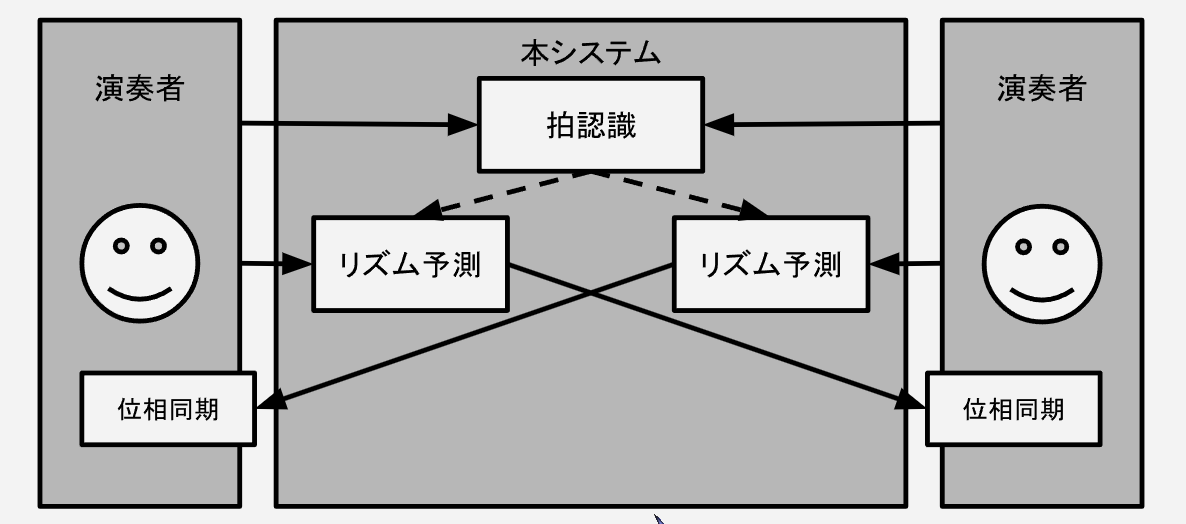
\includegraphics[width=0.8\linewidth]{src/architecture.png}
  \caption{本システムのアーキテクチャ}
  \label{fig:architecture}
\end{figure}


\section{拍認識の実装}
演奏予測を行い,相手の演奏を再生するためには2人の演奏のテンポを知る必要がある.
人間的な誤差,または表現の一環として楽曲を通して演奏のテンポは変化していくため,リアルタイムで直近数秒間の演奏を参照して現在のテンポを認識するアルゴリズムが必要である.
本システムの拍認識では\cite{dixon:2000}で使われたアルゴリズムを用いる.

この拍認識アルゴリズムではDixonのアルゴリズム\cite{dixon}に従って打鍵間隔(Inter-onset interval: IOI)のクラスタリングを行う.
IOIとは任意の2つの音の開始時点の時間間隔のことを指す.
このアルゴリズムの分脈では0.025秒から2.5秒の間のIOIしか扱わず,これより小さいIOIは「同時に鳴った音」として扱う.
ある演奏区間に存在するすべての有効なIOIに対し以下のようにクラスタリングを行う.

\begin{algorithm}
  \caption{Dixon's IOI Clustering Algorithm}
\begin{algorithmic}[1]
\For{each pair of onset times \( t_i, t_j \) with \( t_i < t_j \)}
    \If{\( 0.025 < t_j - t_i < 2.5 \)}
        \State Let \( I = t_j - t_i \)
        \State Find cluster \( C_k \) such that \( | Average ( C_k ) - I | \) is minimum
        \If{\( k \) exists and \( | Average(C_k) - I | < \Delta \)}
            \State \( C_k \gets C_k \cup \{ I \} \)
        \Else
            \State Create new cluster \( C_m := \{ I \} \)
        \EndIf
    \EndIf
\EndFor
\end{algorithmic}
\end{algorithm}

このアルゴリズムでは全クラスタのうち,平均値が最も近いクラスタに対して,その平均値との差が\(\Delta\)以下の場合にのみIOIをクラスタに追加する.

\subsection{共通テンポの算出}
\section{演奏予測の実装}
演奏予測には様々な手法が存在する.

今回は音楽的な表現の伝達に十分な精度しか必要ないため,/cite{tablenet}で用いられた手法を参考にした簡易的な予測手法を用いる.

\begin{figure}[htbp]
  \centering
  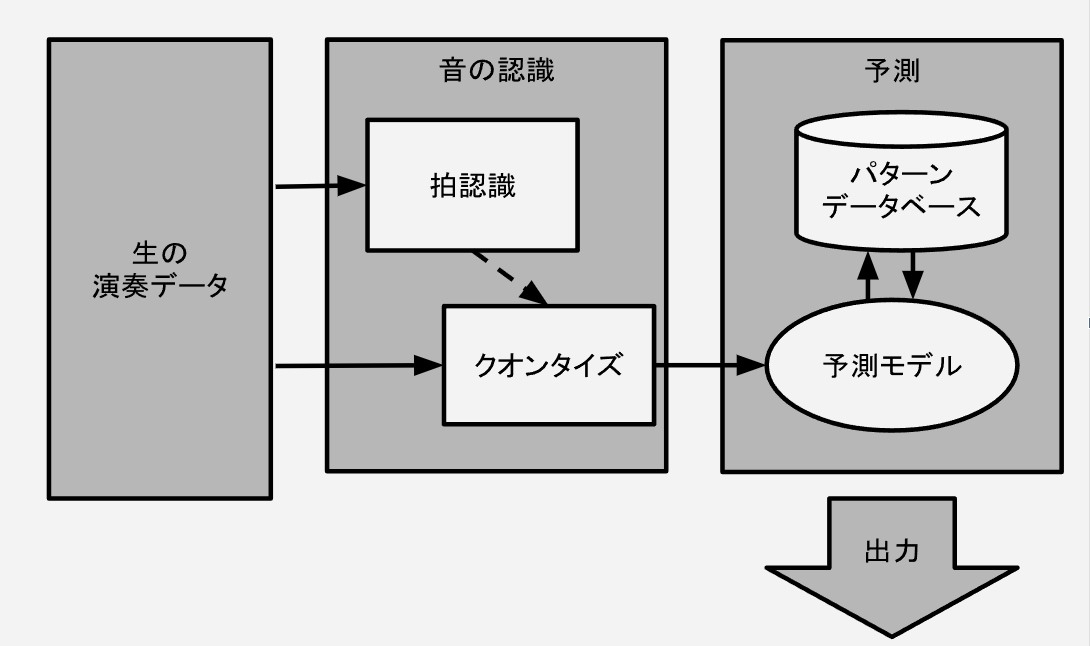
\includegraphics[width=0.8\linewidth]{src/pred.png}
  \caption{予測システム}
  \label{fig:tablenet}
\end{figure}

\section{位相修正}
受信部分において演奏相手の演奏予測を受け取った際,遅延を考慮して位相をずらして再生する必要がある.

\subsection{クロック同期}
OSCタイムタグはUNIX時間を基準にした絶対的な時間で送られるため,各クライアントのわずかな時計のずれで再生時間が変わってしまう.
そのため時計のずれを考慮したタイムタグの修正が必要である.
本システムでは簡易的であり,十分な精度が得られるという理由でCristianのアルゴリズム\cite{cristian}を採用している.

% TODO: 本システムで用いるクロック同期の開設計算式

%%% Local Variables:
%%% mode: japanese-latex
%%% TeX-master: "../bthesis"
%%% End:
